\chapter{Comparison of Knowledge Tracing Methods}

\section{Description of Datasets}\label{sec:kt_data}
We use four publicly available datasets, three of which are standard in the knowledge tracing literature. Two of the four datasets are simulated according to IRT models to demonstrate the capability of our IRT-inspired knowledge tracing methods to learn the IRT model parameters. We also include two real-world datasets common in knowledge tracing literature. A summary of each dataset is given in Table \ref{tab:kt_data}.

\subsubsection*{Synth5}
This dataset \footnote{https://github.com/chrispiech/DeepKnowledgeTracing/tree/master/data/synthetic} was generated by Piech et al. \cite{piech2015} for experiments with DKT. There are 50 items covering 5 latent concepts. Each item requires exactly one concept, and responses are generated according to the Rasch model \cite{lord1968} with guessing: 
\begin{equation}
  P(u_{ij} = 1| \Theta_j; b_i) = c + \frac{1-c}{1 + e^{b_i - \theta_{jk}}}
  \label{eq:rasch_guess}
\end{equation}
The guessing parameter $c$ is fixed at $0.25$. Note that in Equation \ref{eq:rasch_guess}, all items are simple items -- only a single skill $k$ is referenced when answering item $i$. Responses to each of the 50 items are simulated for 4,000 students.

\subsubsection*{Sim200}
Sim200 \footnote{https://github.com/converseg/irt\_data\_repo/tree/master/sim200} differs from Synth5 in a few important ways. First, there are more items (200) and more latent skills (20). Second, the $Q$-matrix is more dense -- items require multiple skills in order for students to answer correctly. Each entry in the $Q$-matrix was sampled from $\text{Bern}(0.2)$. Lastly, Sim200 generates responses according to the ML2P model in Equation \ref{eq:ml2p}, as opposed to the Rasch model. The item parameters were taken from a random uniform distribution; the difficulty parameters from $b_i \in [-3,3]$ and the nonzero discrimination parameters from $a_{ik} \in [0.1,0.9]$. This dataset is very similar to the Sim-20 dataset described in Section \ref{sec:irt_data}, but the latent abilities $\vect \Theta$ were generated according to a standard normal Gaussian distribution.

\subsubsection*{Statics2011}
Statics \footnote{https://pslcdatashop.web.cmu.edu/DatasetInfo?datasetId=507} is a real-world dataset with responses from 316 students enrolled in a college engineering course. After formatting the data (removing a student's multiple attempts on the same item), the dataset includes 987 unique items and 61 latent concepts. Students answered varying amounts of questions, with a total of 135,338 distinct interactions.

\subsubsection*{Assist2017}
The ASSISTments 2017 dataset \footnote{https://sites.google.com/view/assistmentsdatamining} contains real-world interactions from 1,709 students recorded on the ASSISTments online tutoring system. There is a large number of distinct items (4,117), and 102 latent concepts. Some items are tagged with the concept ``noskill'' -- we treat this tag as a distinct latent concept, otherwise all interactions involving such items would need to be thrown out.

\begin{table}
  \centering
  \begin{tabular}{l c c c c}
    \hline
    Dataset & Items & Skills & Students & Interactions \\
    \hline
    Synth5 & 50 & 5 & 4,000 & 20K \\
    Sim200 & 200 & 20 & 50,000 & 10M \\
    Statics2011 & 987 & 61 & 316 & 135K \\
    Assist2017 & 4,117 & 102 & 1,709 & 392K \\
  \end{tabular}
  \caption{Summary of datasets.}
  \label{tab:kt_data}
\end{table}


\section*{Experiment Details}
In the two simulated datasets (Synth5 and Sim200), all students answering the same set of questions and thus all have the same length of response sequences (50 and 200, respectively). For these simulated datasets, the order of responses is shuffled randomly for each student -- the importance of this permuation is discussed in Section \ref{sec:shuffle}. On Statics2011 and Assist2017, the maximum sequence length is set at $L=128$, and a student whose response sequences are longer/shorter than 128 interactions have their response sequences wrapped/padded. The rest of the hyperparameters are described in Table \ref{tab:kt_params}. The hyperparameters for DKT, SAKT, and DKVMN follow those reported in their respective literature \cite{piech2015, pandey2019, zhang2017}.

\begin{table}
  \centering
  \begin{tabular}{l c c c c c}
    \hline
    Parameter & Synth5 & Sim200 & Statics2011 & Assist2017 \\
    \hline
    max\_len & 50 & 200 & 128 & 128 \\
    input\_size & 101 & 201 & 1975 & 8235 \\
    output\_size & 50 & 200 & 987 & 4117 \\
    hid\_size & 64 & 64 & 50 & 100 \\
    skill\_layer & 5 & 20 & 61 & 102 
  \end{tabular}
  \caption{Hyperparameters used in DKT-IRT and SAKT-IRT on each dataset.}
  \label{tab:kt_params}
\end{table}

\section{Quantitative Results} \label{sec:kt_results}

As seen in Table \ref{tab:kt_results}, the two IRT-inspired knowledge tracing methods methods (DKT-IRT and SAKT-IRT) are able to produce AUC values competitive with other deep learning methods. As expected, the sacrifice in accuracy is smaller in simulated datasets. In Synth5 and Sim200, the responses were generated with known IRT models which match the architecture of IRT-inspired methods. 

\begin{table}
  \centering
  \begin{tabular}{l c c c c}
    \hline
    Method & Synth5 & Sim200 & Statics2011 & Assist2017 \\
    \hline 
    DKT & 0.803 & 0.838 & 0.793 & 0.731 \\
    SAKT & 0.801 & 0.834 & 0.791  & 0.754 \\
    DKVMN & 0.827 & 0.829 & 0.805 & 0.796 \\
    \textbf{DKT-IRT} & 0.799 & 0.824 & 0.777 & 0.724 \\
    \textbf{SAKT-IRT} & 0.798 & 0.833 & 0.775 & 0.728
  \end{tabular}
  \caption{TestAUC values for various models on each dataset.}
  \label{tab:kt_results}
\end{table}

Note that when working on Synth5, we know that there were no discrimination parameters used to generate the data. As such, we fix all nonzero weights in the output layer to be equal to one by replacing Equation \ref{eq:weight_constraint} with $W_p \gets Q$. We do not incorporate any estimation or knowledge of the guessing parameter $c$ into the knowledge tracing model. This may account for a larger discrepancy in AUC between our methods and DKVMN in Synth5 than seen in the Sim200 data.

When looking at the two real-world datasets, the trade-off in AUC is more significant, as it is not known if the observed student responses actually follow the ML2P model. There could also be inaccuracies in the given item-skill association $Q$-matrix, which our models are dependent on. Additional difficulties in the Assist2017 data (discussed in Section \ref{sec:kt_data}) concerning exercise-skill tags may explain the considerable performance gap between IRT-inspired methods and DKVMN on this dataset.

\begin{figure}[h]
  \centering
  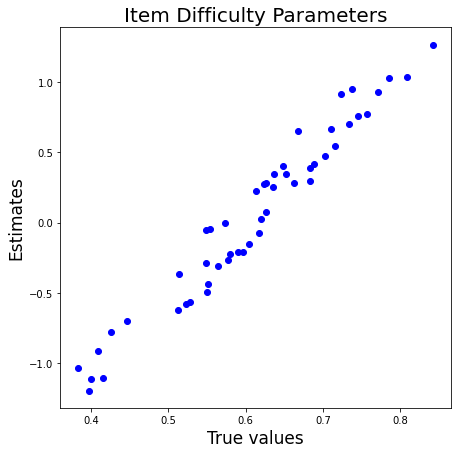
\includegraphics[width=.5\textwidth]{img/kt_irt/synth5_diff_est_lstm.png}
  \caption{Correlation between DKT-IRT estimates and true values of Synth5 item difficulty. SAKT-IRT produced similar results.}
  \label{fig:synth5_diff}
\end{figure}

A comparison between the output layer bias parameters and true item difficulty parameters is shown in Figure \ref{fig:synth5_diff}. This displays high correlation, and the trainable bias parameters in the output layer can be interpreted as approximations of the item difficulty parameters. Due to the available public dataset, there is no access to the true values of student abilities $\vect \Theta$.

\begin{figure}[h]
  \centering
  \minipage{.5\textwidth}
  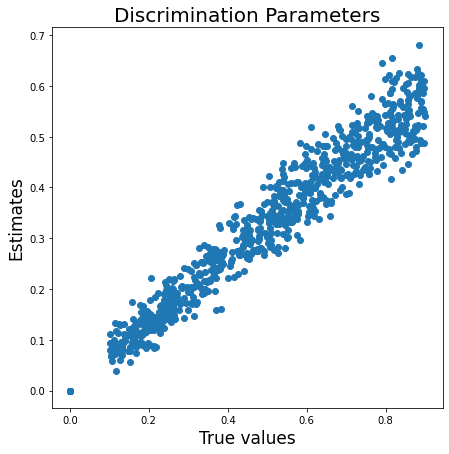
\includegraphics[width=.85\textwidth]{img/kt_irt/disc_est_attn2.png}
  \endminipage
  \minipage{.5\textwidth}
  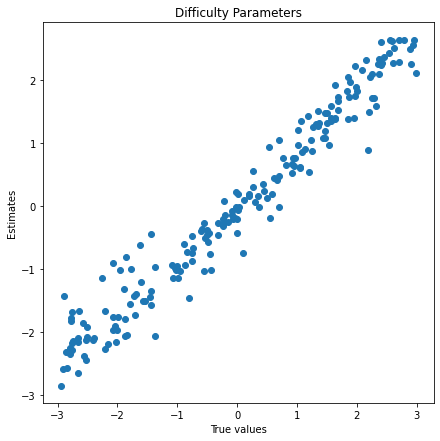
\includegraphics[width=.85\textwidth]{img/kt_irt/diff_attn_sim200.png}
  \endminipage
  \caption{Correlation between true and estimated Sim200 item discrimination parameters (left), and item difficulty parameters (right).}
  \label{fig:disc_diff_sim200}
\end{figure}

The parameter estimates can be directly compared to the true parameters in the Sim200 dataset. In Figure \ref{fig:disc_diff_sim200}, we can see the true values of item discrimination parameters $a_{ik}$ and item difficulty parameter. The correlation here is very high, and the estimates for item parameters are quite accurate. The student ability parameters $\theta_{jk}$ plotted against estimates given by SAKT-IRT at the final timestep in Figure \ref{fig:theta_sim200}. While there is a lot more noise in the student ability estimates, there is still significant correlation with the true values. 

It is important to note that the estimates to $\vect \Theta$ do not require any additional computation or transformation and are directly obtained from a hidden neural network layer. This is an advantage over other deep knowledge tracing methods, which only output the probability of answering items correctly and require other methods of quantifying knowledge concepts. Recall that while estimates to student ability are the neuron activation values at the skill layer from feeding forward a response sequence, the discrimination parameter estimates are the trained weights connecting the skill layer to the output layer, visualized in Figure \ref{fig:kt_irt_visual}.

\begin{figure}[h]
  \centering
  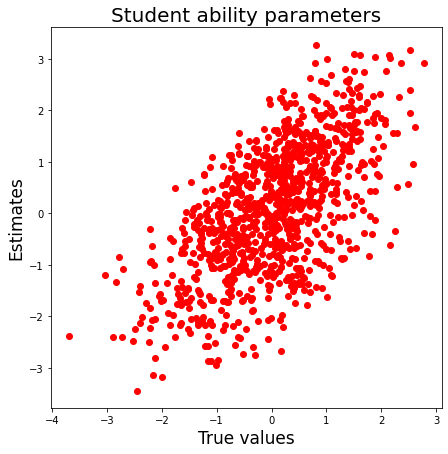
\includegraphics[width=.5\textwidth]{img/kt_irt/theta_est_attn2.png}
  \caption{Correlation between true and estimated student ability parameters at $t=L=200$ for the Sim200 dataset.}
  \label{fig:theta_sim200}
\end{figure}

\begin{figure}[h]
  \centering
  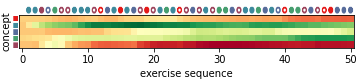
\includegraphics[width=.7\textwidth]{img/kt_irt/knowledge_trace_lstm_edited.png}\\
  \vspace{.5cm}
  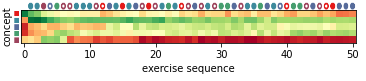
\includegraphics[width=.7\textwidth]{img/kt_irt/knowledge_trace_attn_edited.png}
  \caption{Tracing a student's knowledge mastery with DKT-IRT (top) and SAKT-IRT (bottom) as they progress through the items of the Synthetic-5 dataset.}
  \label{fig:synth5_trace}
\end{figure}

The explcit representation of knowledge $\vect \Theta$ makes tracing student progress over time very convenient. For student $j$'s response sequence of length $L$, IRT-inspired knowledge tracing methods return a $K \times (L+1)$ matrix, where the entry $(k,t)$ gives the latent trait estimate to the $k$-th skill at time $t$, $\theta_{jkt}$. This is visualized in Figure \ref{fig:synth5_trace} on the Synth5 dataset. Notice how a correct response in a skill (filled-in circle) corresponds with a more green and less red skill value. Likewise, an incorrect response in a skill (hollow circle) corresponds with a more red skill or less green skill value. When comparing the knowledge tracing from DKT-IRT and SAKT-IRT, the DKT-IRT tracing is much more smooth as a student moves through the exam. This is likely because of the recurrent structure of an LSTM: the skill values at time $t$ are only directly related to the values at time $t-1$. The SAKT-IRT tracing graphic is much choppier, because the attention mechanism does not have smooth recurrent structure and instead maintains connections to all previous interactions.

\subsection{The Effect of Shuffled Responses}\label{sec:shuffle}
In Section \ref{sec:kt_data}, we mention that the orderings of each student's responses on the simulated datasets were randomly permuted. If all students answer all questions in the same order, then the IRT-inspired knowledge tracing method suffers greatly, particularly when viewing the item parameter estimates. This is due to how student knowledge $\vect \Theta$ is estimated initially at $t=0$, when no other information is provided to the model.

Consider the Sim200 dataset and assume that all students answer all items in the same order ($1, 2, \ldots,199,200$). At $t=0$, all students have the same estimate for their latent traits, $\hat{\theta}_{jk0} = s_{0k}^*$ for all $j$ as in Figure \ref{fig:kt_irt_visual} -- this is a poor estimate of student ability. This skill estimate is multiplied by the weight corresponding to a discrimination parameter of the first item, $w_{1k}q_{1k} = \hat a_{1k}$. 

Since every student answers item 1 first, the same value $s_{0k}^*$ is used in calculating $P(u_{1j} = 1)$ for all $j$. The innacuracy of $s_{0k}^*$ in all cases makes it difficult to estimate $a_{1k}$ -- the same is true for many items appearing early in the fixed response order. In Figure \ref{fig:no_shuffle}, we can compare the discrimination parameter estimates of items early versus late in the response order. Notice that the estimates are much more correlated with the true values for items towards the end of the sequence, since they have access to a more accurate estimate of each student's latent ability $\hat \theta_{jkt}$.

\begin{figure}[h]
  \centering
  \minipage{.5\textwidth}
  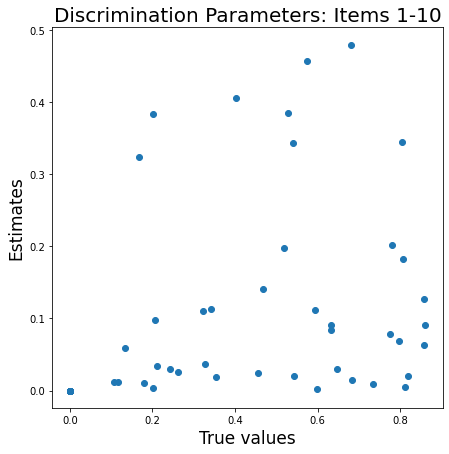
\includegraphics[width=.8\textwidth]{img/kt_irt/disc_est_no_shuffle_early.png}
  \endminipage
  \minipage{.5\textwidth}
  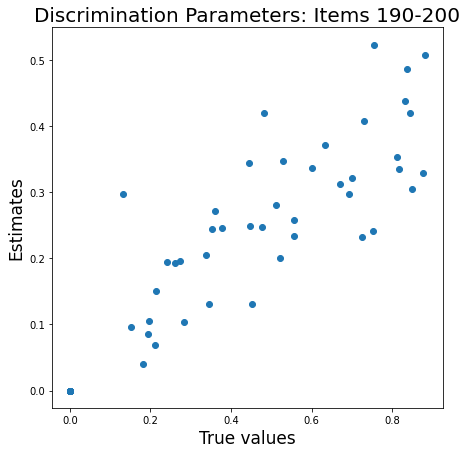
\includegraphics[width=.8\textwidth]{img/kt_irt/disc_est_no_shuffle_late.png}
  \endminipage
  \caption{Discrimination parameter estimates of items early in the response sequence (left) and items late in the response sequence (right) when all students answer items in the same order.}
  \label{fig:no_shuffle}
\end{figure}

\subsection{Using Attention to Learn Item-Skill Associations}
An advantage of other knowledge tracing methods such as DKT is that it does not require any expert annotation of the item-skill association. In other words, the only required data is the student response sequences, and not a $Q$-matrix. In the IRT-inspired knowledge tracing methods described in Chapter \ref{ch:kt_methods}, this $Q$-matrix is required to build the architecture used for the results reported in Section \ref{sec:kt_results}.

Multiple methods of discovering item-skill relationships from deep models have been proposed in the literature. For example, Piech et al. \cite{piech2015} proposes calculating the conditional influence between each item for this task. This involves finding the relative change that a correct response on item $i$ has on the probability of answering item $j$ correctly, computed by feeding the corresponding response sequences through DKT. In DKVMN \cite{zhang2017}, the correlation weights $\vect w_t$ from Equation \ref{eq:dkvmn_weight} are used to quantify the relationship between items and memory slots. A similar approach is used by Pandey et al. in SAKT \cite{pandey2019}, using the attention weight in Equation \ref{eq:attn_sakt} to relate each interaction in a response sequence.

We follow the framework of SAKT and use the attention mechanism to discover a $Q$-matrix. When using the SAKT-IRT architecture but removing the $Q$-matrix constraint, we arrive at a knowledge tracing framework that is nearly identical to SAKT. After training on the Synth5 dataset, we feed-forward a response sequence of a student answering all 50 items correctly After training on the Synth5 dataset, we feed-forward a response sequence of a student answering all 50 items correctly and calculated the correlation weights similar to Equation \ref{eq:attn_sakt}:
\begin{equation}
  \vect w_t = \text{softmax}\left(\frac{K \vect q_t}{\sqrt{d}} \right), \quad 0\leq t \leq 50
  \label{eq:q_cor_weights}
\end{equation}

We can arrange all correlation vectors $\vect w_t$ into a single matrix $C \in \R^{51 \times 51}$. A heatmap of $C$ is shown in Figure \ref{fig:attn_item_cor}. Note that the upper-right half of $C$ is all zero -- this is due to masking out future interactions (interaction $t$ cannot draw inferences from interaction $t+1$).
\begin{figure}[h]
  \centering
  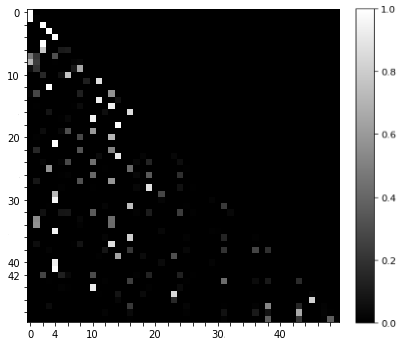
\includegraphics[width=.65\textwidth]{img/kt_irt/synth5_attn_weights_no_ffn_axis2.png}
  \caption{Heatmap of the item correlation matrix $C$, where each row quantifies the relationship between an item and all previous items, starting in the top-left corner.}
  \label{fig:attn_item_cor}
\end{figure}
The sum of each row of $C$ is equal to 1, and each entry in row $i$ can be interpreted as the relevance between each previous interaction and item $i$. For example, item 42 draws some information from previous interactions 2, 5, 10, 19, and 24, seen in row 42. In a similar manner, item 4 is heavily relied upon for reference when querying interactions 21, 29, 30, 35, 40, and 41, seen in column 4.

The natural assumption is that items which are correlated by Equation \ref{eq:q_cor_weights} measure the same latent concept. To better visualize the item-skill association, we construct a weighted graph $G$, with each node representing an item and edge weights determined by the symmetric matrix $C + C^\top - \text{diag}(C)$. Using the NetworkX library for Python \cite{networkx}, we use a force-directed algorithm to visualize $G$ in 2-D space. This algorithm places node pairs with heavier weighted edges between them closer together \cite{fruchterman1991}, resulting in a clustering of items which are similar.

\begin{figure}[h]
  \centering
  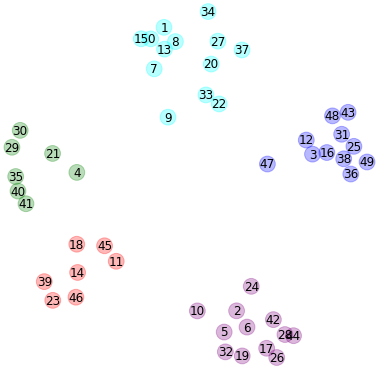
\includegraphics[width=.55\textwidth]{img/kt_irt/synth5_clusters_no_ffn.png}
  \caption{Visualization of the graph $G$, showing a five clusters of items which correspond to the five concepts in the Synth5 dataset.}
  \label{fig:synth5_clusters}
\end{figure}
The graph $G$ is shown in Figure \ref{fig:synth5_clusters}. The different colors identify the true skill tag of each item -- this information was provided to neither the neural network nor the graph visualization algorithm. NetworkX was not even provided the number of skills, yet still arranges the nodes into five distinct clusters. Notice that all items of similar skill are clustered together, displaying that the correlation matrix $C$ in Figure \ref{fig:attn_item_cor} does in fact learn the item-skill associations. For example, items 42 and 4 are both found in clusters along with the items mentioned ealier which share larger values in $C$. The visualization of the graph $G$ can be used to build a $Q$-matrix for use in DKT-IRT or SAKT-IRT, as described in Section \ref{sec:kt_irt_methods}.

\section{Discussion}

\subsection{Future Extensions} \sideremark{TODO -- missing data framework, Q-matrix in attn calc}


\subsection{Concluding Remarks}
The connection between IRT and knowledge tracing presented in this work introduces a trade-off between accuracy and interpretability. Further work to increase AUC to the level of DKVMN while maintaining explainability is worth exploring. Though IRT-inspired knowledge tracing does require an expert to annotate the item-skill association $Q$-matrix while other methods do not, explicitly incorporating this domain knowledge greatly increases the ability to interpret a deep learning model. Further, most intelligent tutoring systems provide an item-skill tag, so availability of the $Q$-matrix is not an unreasonable assumption.

Our proposed method's ability to function as both a knowledge tracing model while also estimating item parameters gives it a unique interpretation rooted in Item Response Theory. This link with IRT is helpful in practice, because it provides an explicit and easy to obtain quantity for a student's latent abilities. The approximation of a student ability can be interpreted in the frame of IRT, as opposed to only a prediction of correctness for each item. This is a clear advantage that IRT-inspired knowledge tracing has over conventional non-interpretable deep learning methods in knowledge tracing.

